\documentclass[noamssymb,svgnames]{beamer}
\usecolortheme{beaver}
\useinnertheme[shadow]{rounded}
\usefonttheme{serif}
\usefonttheme{professionalfonts}

\usepackage[bitstream-charter]{mathdesign} % Use BT Charter font
\usepackage[T1]{fontenc}                   % Use T1 encoding instead of OT1
\usepackage[utf8]{inputenc}                % Use UTF8 input encoding
\usepackage{microtype}                     % Improve typography
\usepackage{booktabs}
\usepackage[binary-units]{siunitx}
\usepackage{tikz}
\usetikzlibrary{shapes.geometric}

\usepackage{hyperref}
\hypersetup{pdfstartview=Fit}

% BEAMER CONFIGURATION ---------------------------------------------------------
\setbeamerfont{block title}{size=\normalsize}
\setbeamerfont{block body}{size=\scriptsize}
\setbeamercolor{block title}{fg=darkred,bg=gray!10!white}
\setbeamercolor*{item}{fg=darkred}

% TCOLORBOX / MINTED CONFIGURATION ---------------------------------------------
\usepackage[many,minted]{tcolorbox}
\NewTCBListing{python}{ O{} }{listing only,minted language=python,#1}
\setminted{
  mathescape,
  autogobble,
  fontfamily=courier,
  framesep=2mm
}


\newcommand\blfootnote[1]{%
  \begingroup
  \renewcommand\thefootnote{}\footnote{#1}%
  \addtocounter{footnote}{-1}%
  \endgroup
}

% ------------------------------------------------------------------------------
\title{Temperature Dependence}

\institute{
\includegraphics[width=2in]{../images/openmc_logo.png}}

\date{OpenMC Workshop \\ Canadian Nuclear Laboratories \\ March 14--16, 2017}

% ------------------------------------------------------------------------------
\begin{document}

\frame{\titlepage}

% ------------------------------------------------------------------------------

\begin{frame}{Temperature Dependence}
  \begin{itemize}
  \item Reactor analysis requires at-power temperature distribution $\to$ cross
    sections needed for all temperatures
  \item Approaches:
    \begin{enumerate}
    \item Brute force: store cross sections at a finite number of temperatures
      and interpolate between them as needed (memory may approach 100s of GB)
    \item Polynomial expansion (Yesilyurt and Martin): Express dependence of
      temperature for a given cross section at a given energy as a polynomial
      expansion
    \item Target motion sampling (Viitanen and Leppanen): introduces a rejection
      sampling step each time neutron moves, only requires \SI{0}{\kelvin} data
    \end{enumerate}
  \end{itemize}
\end{frame}

\begin{frame}{Windowed Multipole Method\blfootnote{
      \textit{J. Comput. Phys.}, \textbf{307}, 715 (2016)}}
  \begin{itemize}
  \item R. Hwang (ANL) introduced a multipole formalism for representing
    resonance cross sections
  \item Revisited/reformulated by Forget/Josey (MIT) to take advantage of
    analytic form of Doppler broadening
    \begin{align*}
      \sigma(u,0) &= \frac{1}{u^2} \sum\limits_j \Re \left [ \frac{r_j}{p_j - u}
        \right ] \\ \sigma(u,T) &= \frac{1}{2u^2\sqrt{\xi}} \sum\limits_j \Re
      \left [ ir_j \sqrt{\pi} W(z_j^0) - \frac{r_j}{\pi} C\left (
        \frac{p_j}{\sqrt{\xi}}, \frac{u}{2\xi} \right ) \right ]
    \end{align*}
  \item Need to store poles/residues for each resonance of nuclide
  \item Cross section evaluation becomes FLOP-dominated rather than
    memory-latency dominated
  \end{itemize}
\end{frame}

\begin{frame}{Windowed Multipole Method}
  \begin{center}
    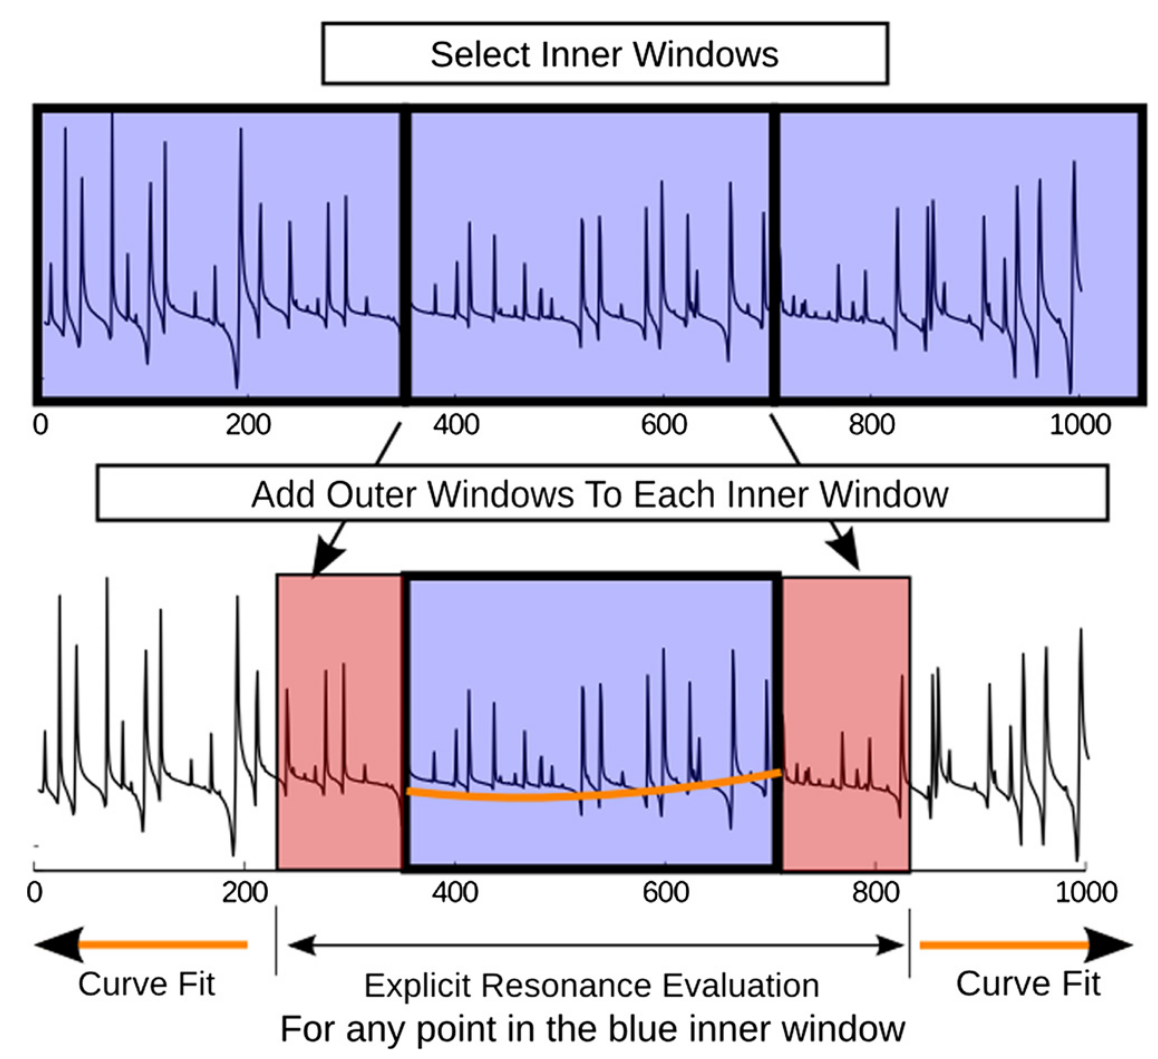
\includegraphics[width=3in]{../images/windowed_multipole.png}
  \end{center}
\end{frame}

\end{document}
